\section{Segmentation by thresholding}
\subsection{Histogram-based segmentation}

The implementation is pretty trivial, but in any case, here is a snippet of the
function I use for thresholding:

\begin{minted}[linenos=true]{python}
def threshold(img, th):
    return np.uint8(img > th)
\end{minted}

\Cref{fig:4.1} shows the binary segmentation using thresholding with \texttt{th}
= 100. We successfully segmented the objects in the image, however we also
picked up a lot up noise from light spots in the fabric in the background of the
image, so \emph{no}, we did not succeed in completely separating the foreground
objects from the background with simply thresholding.

\begin{figure}[H]
    \centering
    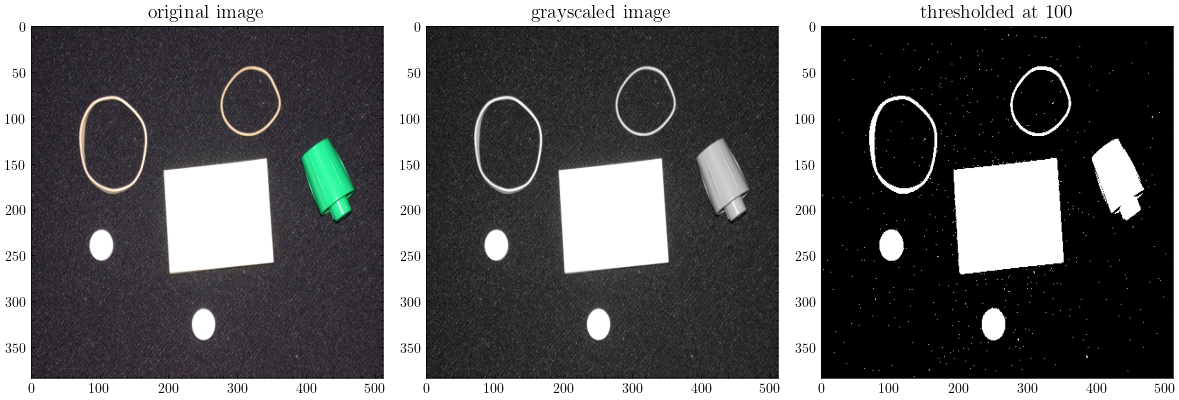
\includegraphics[width=\textwidth]{figures/task_4_1.png}
    \caption{Original image, grayscale image, and my binary segmentation.}
    \label{fig:4.1}
\end{figure}


\subsection{Inspecting the histogram}

\Cref{fig:4.2} shows the histogram of the grayscale image. The majority of
pixels lie in a bell curve in \emph{roughly} the range 25..100, but there also
is a very big concentration of pixels of value 255. This peak at 255 is likely
from the white square and the two pills, which in the color image are the only
completely white objects. The histogram is nearly zero, but not completely zero
between 100 and 255, and these pixel values likely represent the rubber bands
and the green object in the original image.


The bell curve in the range 25..100 is centered roughly at 50, and thus likely
represents the dark background. For this reason the chosen threshold of 100 was
a very good choice of threshold for this particular image. By visual inspection
of the original image, we see that the fabric in the background contains a lot
of small ``specks'' of light threads, which may be hard (or impossible) to
remove using thresholding without also losing details in eg. the green object,
which has some dark features, so even if the optimal threshold is not 100, then
it is probably very close to 100.

\begin{figure}[H]
    \centering
    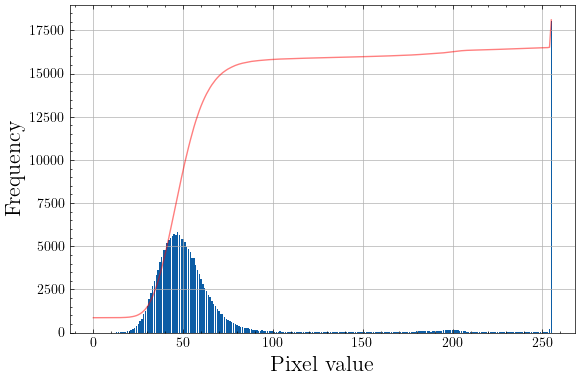
\includegraphics[width=0.8\textwidth]{figures/task_4_2.png}
    \caption{Original image, grayscale image, and my binary segmentation.}
    \label{fig:4.2}
\end{figure}

